\documentclass[tikz, border=3mm]{standalone}
\usepackage{tikz}
\usepackage{amsmath} % For math symbols if needed
\usepackage{amssymb} % For math symbols if needed
\usetikzlibrary{positioning} % For label positioning

\begin{document}
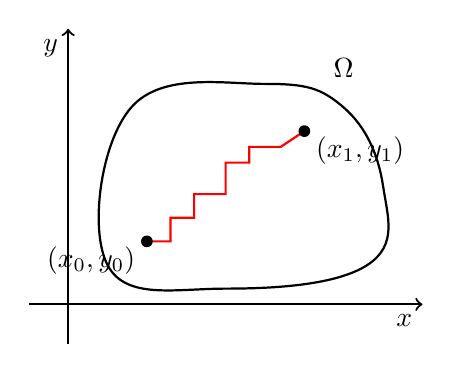
\begin{tikzpicture}[
    point/.style={fill=black, circle, inner sep=1.5pt} % Style for points
]

% Axes
\draw[->, thick] (-0.5, 0) -- (4.5, 0) node[below left] {$x$};
\draw[->, thick] (0, -0.5) -- (0, 3.5) node[below left] {$y$};

% Outer Blob - using plot smooth cycle for approximation
\draw[thick] plot [smooth cycle, tension=0.7] coordinates {
    (0.5, 0.5) (0.8, 2.5) (2.5, 2.8) (3.5, 2.5) (4.0, 1.5) (3.8, 0.5) (2.0, 0.2)
};

% Region Label
\node at (3.5, 3.0) {$\Omega$};

% Define Start and End Points
\coordinate (start) at (1.0, 0.8);
\coordinate (end) at (3.0, 2.2);

% Draw Staircase Path (Manhattan path)
\draw[red, thick] (start)
    -- ++(0.3, 0)  % Step right
    -- ++(0, 0.3)  % Step up
    -- ++(0.3, 0)  % Step right
    -- ++(0, 0.3)  % Step up
    -- ++(0.4, 0)  % Step right
    -- ++(0, 0.4)  % Step up
    -- ++(0.3, 0)  % Step right
    -- ++(0, 0.2)  % Step up
    -- ++(0.4, 0)  % Step right (reaches x=3.0)
    -- (end);      % Final vertical segment to end point y

% Mark and Label Start and End Points (Draw last to be on top)
\node[point, label={[below left=1pt of start]$(x_0, y_0)$}] at (start) {};
\node[point, label={[below right=1pt of end]$(x_1, y_1)$}] at (end) {};

\end{tikzpicture}
\end{document}